\documentclass[12pt]{article}
\usepackage[utf8]{inputenc}
\usepackage[russian]{babel}
\usepackage{amsmath}
\usepackage{amssymb}
\usepackage{geometry}
\usepackage{graphicx}
\geometry{a4paper, margin=1in}
\usepackage{listings}
\usepackage{xcolor}
\usepackage[usenames]{hyperref}

\lstset{
  language=C++,                % Язык программирования
  basicstyle=\ttfamily\small,  % Шрифт и размер текста
  keywordstyle=\color{blue},   % Цвет ключевых слов
  commentstyle=\color{gray},   % Цвет комментариев
  stringstyle=\color{red},     % Цвет строк
  numbers=left,                % Нумерация строк слева
  numberstyle=\tiny\color{gray}, % Стиль номеров строк
  stepnumber=1,                % Интервал нумерации строк
  breaklines=true,             % Перенос длинных строк
  frame=single,                % Рамка вокруг кода
}

\title{Отчёт по расчётной работе по дисциплине ПиОИвИС}
\author{}
\date{}


\begin{document}

\maketitle

\begin{center}
\section*{Графы}
\end{center}

\subsection*{Цель}
Определить число рёберной связности путём создания алгоритма, который будет создавать граф по заданным параметрам и вычислять сколько нужно удалить рёбер, чтобы он перестал быть связным.

\subsection*{Вариант}
7.2 (мc,нг)

\section*{Определения}

\begin{itemize}
    \item \textbf{Граф} —  математическая абстракция реальной системы любой природы, объекты которой обладают парными связями. Граф как математический объект есть совокупность двух множеств — множества самих объектов, называемого множеством вершин, и множества их парных связей, называемого множеством рёбер. Элемент множества рёбер есть пара элементов множества вершин.
    
    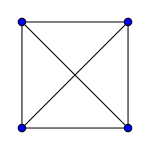
\includegraphics[width=0.4\textwidth, height=3cm, keepaspectratio]{g.png}
    
    \item \textbf{Связный граф} — это граф, у которого две любые вершины соединены путём.
    
     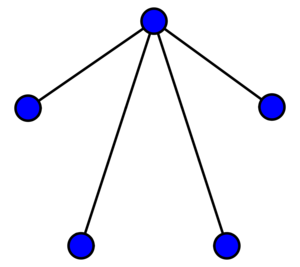
\includegraphics[width=0.7\textwidth, height=5cm, keepaspectratio]{sg.png}

     \item \textbf{Несвязный граф} — граф, содержащий более одной компоненты связности.
    
     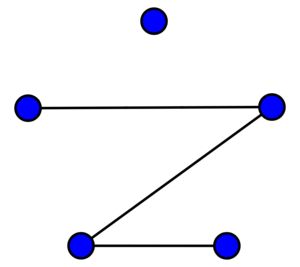
\includegraphics[width=0.7\textwidth, height=5cm, keepaspectratio]{nsg.png}

      \item \textbf{Ориентированный граф} — это граф, рёбра которого ориентированы, то есть имеют начальную вершину и концевую вершину.
    
     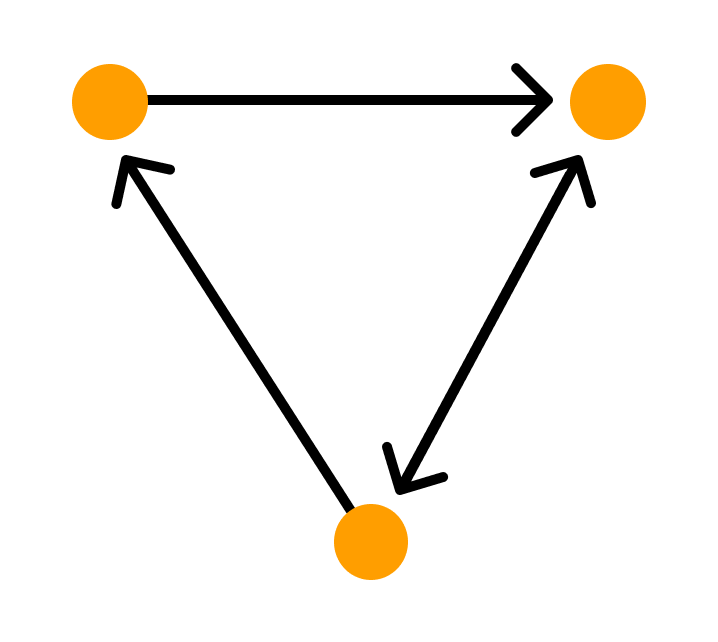
\includegraphics[width=0.7\textwidth, height=5cm, keepaspectratio]{og.png}

      \item \textbf{Неориентированный граф} — графы, в которых все ребра являются звеньями, то есть порядок двух концов ребра графа не существенен.
    
     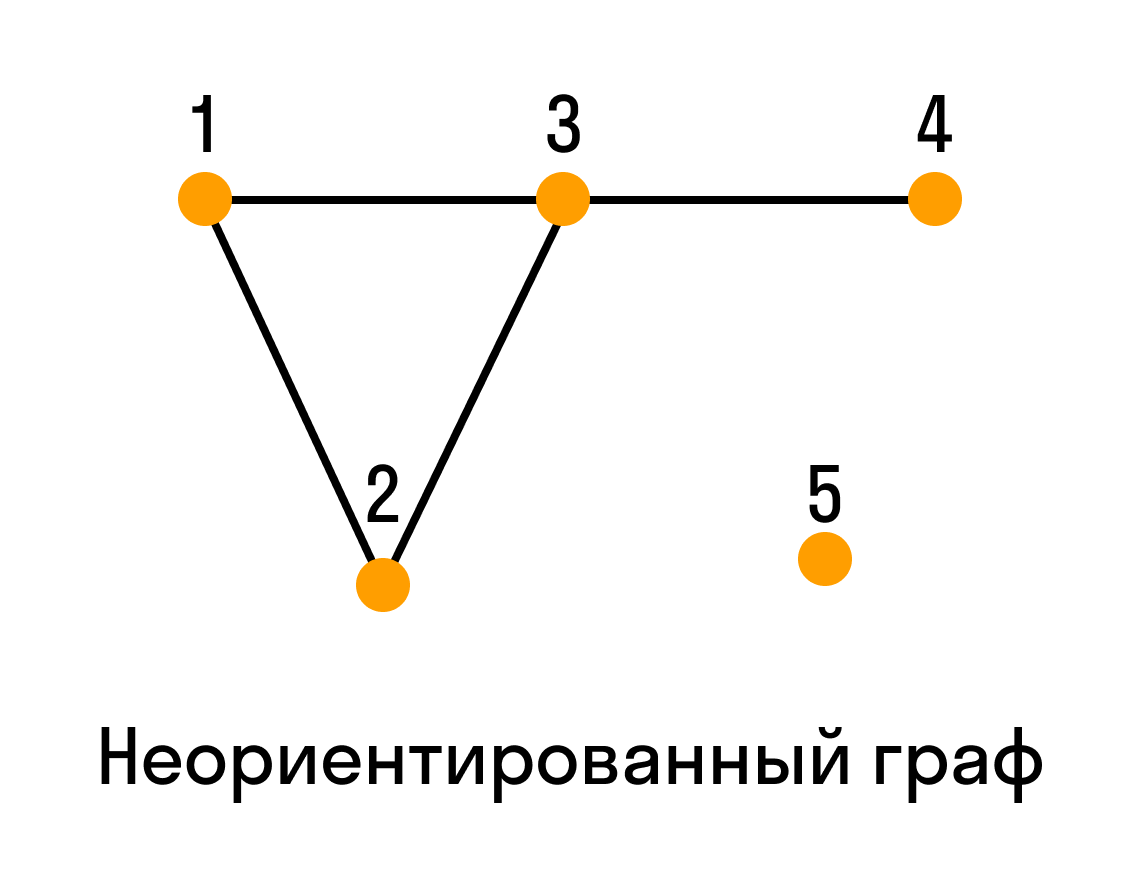
\includegraphics[width=0.7\textwidth, height=5cm, keepaspectratio]{nog.png}
     
    \item \textbf{Сме́жность} — непосредственная близость, примыкание. В теории графов смежность вершин соответствует наличию ребра между ними.
    
    \item \textbf{Матрица смежности} - это вид представления графа в виде матрицы, когда пересечение столбцов и строк задаёт дуги.
    
        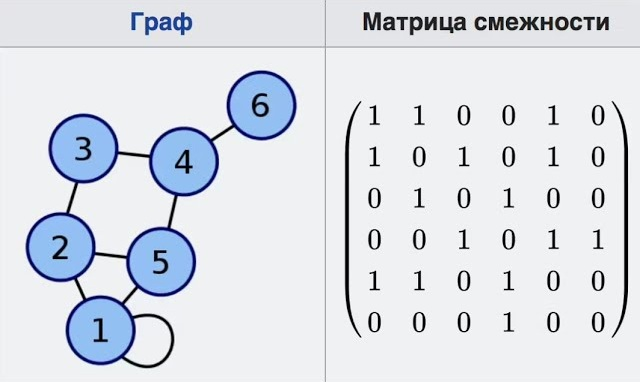
\includegraphics[width=0.5\textwidth, height=4cm, keepaspectratio]{ms.png}
        
\end{itemize}

\section*{Алгоритм}
\begin{enumerate}
    \item Ввести количество вершин.
    \item Ввести количество рёбер.
    \item Ввести сами рёбра.
    \item Совершить поиск вглубь через dfs и пометить посещённые вершины.
    \item Если были посещенны все вершины, то граф - связный. В противном случае - несвязный.
    \item Пройтись по графу путё удаления и восстановления каждого ребра.
    \item Определить минимальное число рёбер, которые нужно удалить что граф из связного превратился в несвязный.
    \item Вывести сообщение: "Минимальное количество рёбер, которые нужно удалить для разъединения графа: ".
\end{enumerate}
\section*{Код}
\begin{lstlisting}
#include <iostream>
#include <vector>
using namespace std;

class Graph {
public:
    int V;
    vector<vector<int>> adj;

    Graph(int V) {
        this->V = V;
        adj = vector<vector<int>>(V, vector<int>(V, 0));
    }

    void addReb(int u, int v) {
        adj[u][v] = 1;
        adj[v][u] = 1;
    }

    void DFS(int v, vector<bool>& visited) {
        visited[v] = true;
        for (int i = 0; i < V; i++) {
            if (adj[v][i] && !visited[i]) {
                DFS(i, visited);
            }
        }
    }

    bool isCon() {
        vector<bool> visited(V, false);
        DFS(0, visited);
        
        for (int i = 0; i < V; i++) {
            if (!visited[i]) return false;
        }
        return true;
    }

    int minRebToRem() {
        int RebRem = 0;

        for (int u = 0; u < V; u++) {
            for (int v = u + 1; v < V; v++) {
                if (adj[u][v]) {
                    
                    adj[u][v] = 0;
                    adj[v][u] = 0;
                    
                    if (!isCon()) {
                        RebRem++;
                    }
                    adj[u][v] = 1;
                    adj[v][u] = 1;
                }
            }
        }
        return RebRem;
    }
};

int main() {
    int V, E;
    cout << "Enter number of vertices: ";
    cin >> V;
    Graph g(V);

    cout << "Enter number of edges: ";
    cin >> E;

    cout << "Enter edges (u v):" << endl;
    for (int i = 0; i < E; i++) {
        int u, v;
        cin >> u >> v;
        g.addReb(u, v);
    }

    int result = g.minRebToRem();
    cout << "Minimum number of edges that need to be removed to disconnect a graph: " << result << endl;
    return 0;
}

\end{lstlisting}
\section*{Примеры работы кода}
\par №1
 \par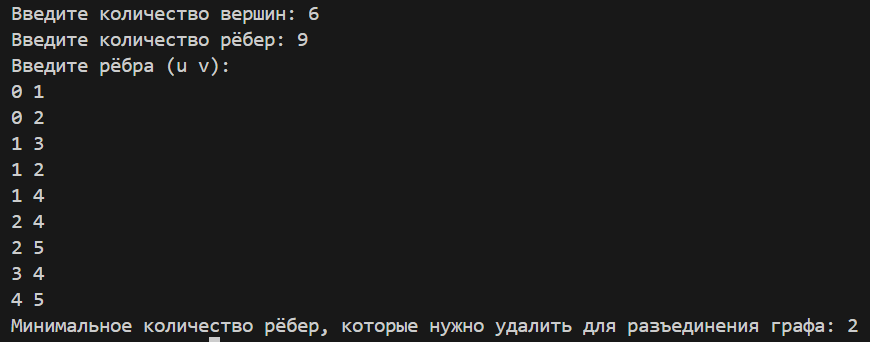
\includegraphics[width=0.9\textwidth, height=12cm, keepaspectratio]{res1.png}
\par №2
 \par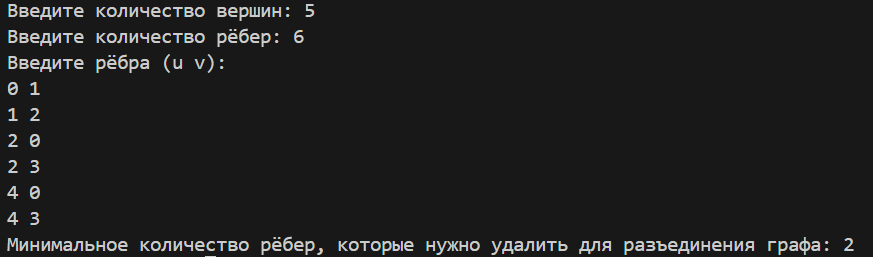
\includegraphics[width=0.9\textwidth, height=12cm, keepaspectratio]{res2.png}
\par №3
\par 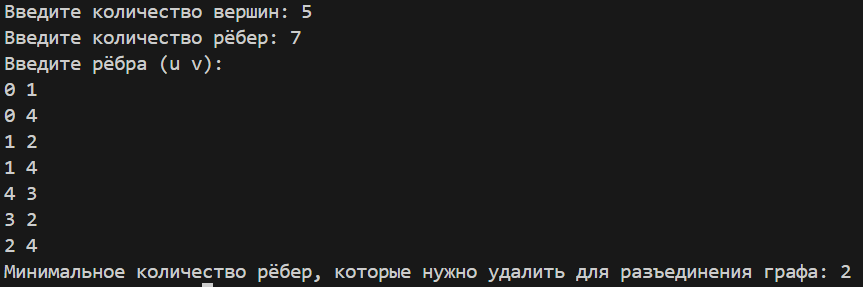
\includegraphics[width=0.9\textwidth, height=12cm, keepaspectratio]{res3.png}
\par №4
\par 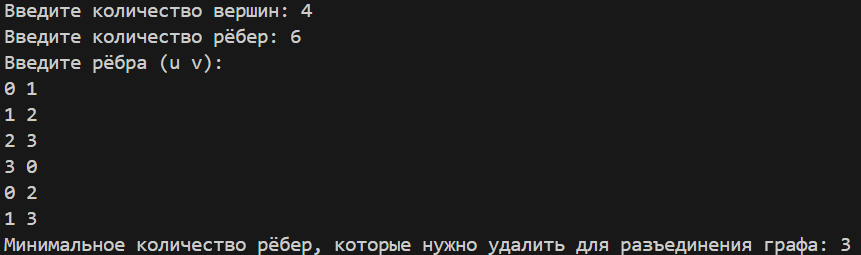
\includegraphics[width=0.9\textwidth, height=12cm, keepaspectratio]{res4.png}
\par №5
 \par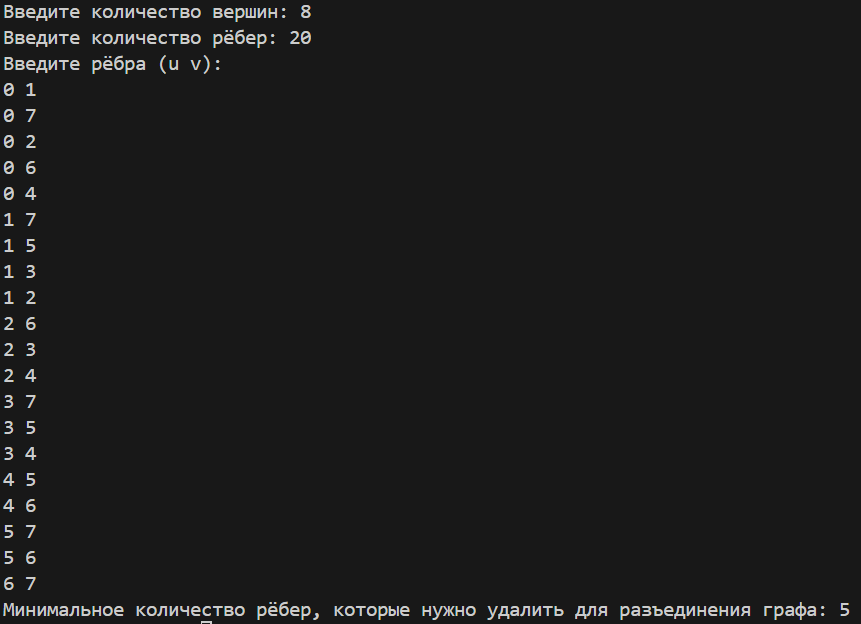
\includegraphics[width=0.9\textwidth, height=12cm, keepaspectratio]{res5.png}
\section*{Вывод}

В результате выполнения данной работы были получены следующие практические навыки:

\begin{itemize}
    \item Изучены основы теории графов.
    \item Изучены способы представления графов.
    \item Изучены базовые алгоритмы для работы с графами.
\end{itemize}

Источники:
\par 
\href{https://skysmart.ru/articles/mathematic/osnovnye-ponyatiya-teorii-grafov}{\textcolor{blue}{https://skysmart.ru/articles/mathematic/osnovnye-ponyatiya-teorii-grafov}}
\par 
\href{https://skyeng.ru/magazine/wiki/it-industriya/chto-takoe-graf/}{\textcolor{blue}{https://skyeng.ru/magazine/wiki/it-industriya/chto-takoe-graf/}}
\par 
\href{https://habr.com/ru/companies/otus/articles/568026/}{\textcolor{blue}{https://habr.com/ru/companies/otus/articles/568026/}}
\par 
\href{https://skillbox.ru/media/code/teoriya-grafov-derevya-planarnost-raznovidnosti-grafov/}{\textcolor{blue}{https://skillbox.ru/media/code/teoriya-grafov-derevya-planarnost-raznovidnosti-grafov/}}
\end{document}